\documentclass[main]{subfiles}
\begin{document}

%@@@@@@@@@@@@@@@@@@@@@@@@@@@@@@
% summarizes lecture 
% author:

\section{Support Vector Machines}
This is the chapter on Support Vector Machines.
\subsection{Lagrangian optimization theory}
\paragraph{Overview}
An Optimization Problem is given by a function which we want to minimize and some constraints:
\begin{align}
minimize \ f(w) \\
subject \ to \ g_i(w) \leq 0, \forall_i \\
and \ h_j(w) = 0, \forall_j
\end{align}
\paragraph{Equality constraints}
Equality constraints define sub-manifolds in the solution space on which the minimal solution has to be located, which is the same as saying that an equation $h(w)=0$ is a (D-1)-dimensional surface in the solution space of w.
At any point on the constraint surface, $\nabla h(w)$ will be orthogonal to the $h(w)=0$ surface. 
\newline
Proof: Consider a point w on the constraint surface and a nearby point $w+\epsilon$ also on the surface. Making a Taylor Expansion around w, we get
\begin{align}
h(w+\epsilon) \simeq h(w)+\epsilon^T \nabla h(w)
\end{align}
Because both points are on the constraint surface, we have $h(w)=h(w+\epsilon) \Rightarrow \epsilon^T \nabla h(w) \simeq 0$. In the limit $\parallel \epsilon \parallel \rightarrow 0$ we have $\epsilon^T \nabla h(w) = 0$ and because $\epsilon$ is parallel to the surface $h(w)$, $\nabla h(w)$ is normal to the surface. \newline
Next we seek a point $w^*$ so that $f(w)$ is minimized. Such a point must have the property that $\nabla f(w)$ is also orthogonal to the constraint surface, because otherwise we would increase the value of $f(w)$ by moving a short distance along along the surface. Thus $\nabla f$ and $\nabla h$ are parallel (or antiparallel) vectors and there's a solution for $\nabla f + \beta \nabla h = 0$ where $\beta$ is a lagrange multiplier. 
\newline
For equality constraints $\beta$ may be positive as well as negative. We now introduce Lagrange functions, first for the simple case with one equality constraint:
\begin{align}
L(w,\beta)=f(w)+\beta h(w)
\end{align}
The constrained stationary condition is obtained by setting $\nabla_w L=0$. Furthermore, the condition $\frac{\partial L}{\partial \beta} = 0$ leads to the constrained equation $h(w)=0$:
\begin{align}
\frac{\partial L}{\partial \beta}=h(w)=0
\end{align}
Thus, to find the minimum of $f(w)$ subject to $g(w)=0$ we take $L(w,\beta)$ and find a stationary point of it with respect to $w$ and $\beta$.
\newline
With a 2-D $w$ we get three equations with three variables:
\begin{align}
\frac{\partial L}{\partial w_1}=0 \\
\frac{\partial L}{\partial w_2}=0 \\
\frac{\partial L}{\partial \beta}=0
\end{align}
Solve equations to find $w^*$ and $\beta$. If only interested in $w^*$ we can eliminate $\beta$ from the equations and solve for $w^*$ directly. In this case the lagrange multipliers are also called undetermined multipliers.
\paragraph{Inequality Constraints}
Now we extend the concept with inequality constraints in the form $g(w) \geq 0$. There are two kinds of solutions possible:
\begin{itemize}
	\item With an inactive constraint $g(w) > 0$
	\item With an active constraint $g(w) = 0$
\end{itemize}
The inactive case corresponds to a solution which ignores the constraint:
\begin{align}
L(w,\alpha)=f(w)+\alpha g(w) \ with \ \alpha=0 \Rightarrow \nabla f(w)=0
\end{align}
The active case corresponds to the case of the equality constraint with $\alpha \neq 0$. Now however the sign of the lagrange multiplier (i.e. $\alpha$) matters because $f(w)$ will only be at its maximum if the gradient $\nabla f(w)$ is oriented away from the region $g(w)>0$. We therefore have:
\begin{align}
\nabla f(w)=-\alpha \nabla g(w) \ for \ \alpha > 0
\end{align}
In both cases, the active and inactive, the following holds: $\alpha g(w)=0$ \newline
Thus, by optimizing 
\begin{align}
L(w,\alpha)=f(w)+\alpha g(w) \\
subject \ to \ g(w) \geq 0 \\
\alpha \geq 0 \\
\alpha g(w) = 0
\end{align}
we find our solution. The three constraints given here are known as the \textbf{Karush-Kuhn-Tucker (KKT) conditions}.
\paragraph{Dual Problem}
Finally we can come up with an equation containing several constraints of both types:
\begin{align}
L(w,\alpha,\beta)=f(w)+\sum_i \alpha_i g_i(w)+\sum_j \beta_j h_j(w) \\
subject \ to \ \alpha_i \geq 0 \ \forall_i \\
\alpha_i g_i(w)=0 \ \forall_i
\end{align}

Steps: 
\begin{enumerate}
	\item Find $w^*$ of $L(w, \alpha, \beta)$ by $\frac{\partial L}{\partial w}\rvert_{w=w^*}=0$
	\item Insert $w^*$ into $L$ and find $\beta^*$ by $\frac{\partial L}{\partial \beta}\rvert_{\beta=\beta^*}=0$
	\item Calculate $\alpha$ by solving the above optimization problem with $w^*$ and $\beta^*$
\end{enumerate}

The \textbf{Dual Problem} given by
\begin{align}
max \theta(\alpha, \beta) \\
subject \ to \ \alpha_i \geq 0 \ \forall_i \\
where \ \theta(\alpha, \beta)=inf_w L(w, \alpha, \beta)
\end{align}
has an upper bound:
\begin{align}
\theta(\alpha, \beta)=inf_u L(u, \alpha, \beta) \leq L(w, \alpha, \beta)=f(w)+\sum_i \alpha_i g_i(w) + \sum_j \beta_j h_j(w) \leq f(w)
\end{align}
Feasibility of w implies $g_i(w)\leq 0$ and $h_j(w)=0$. \newline
Feasibility of $\alpha$ and $\beta$ implies $\alpha_i \geq 0$. \newline
Therefore the first sum is negative or zero and the second one is zero.\newline
\paragraph{Duality Gap}
The optimal solution of the Dual Problem is also called the \textbf{value of the problem}.
The value of the dual problem is upper bounded by the value of the primal problem:
\begin{align}
sup\{\theta(\alpha,\beta): \alpha \geq 0 \} \leq inf \{f(w): g(w) \leq 0, h(w) = 0\}
\end{align}
The difference between the two is called the \textbf{duality gap}. The solution $(w^*, \alpha^*, \beta^*)$ is a saddle point of Lagrangian for the primal problem if and only if its components are optimal solutions of the primal and dual problem and if there's no duality gap. \newline
Given an optimization problem with convex $f$ and convex domain of $w \in \omega \subseteq \mathbb{R}$ and with $g_i$ and $h_j$ that are affine functions, i.e. $g(w)=Aw-b$ for some matrix $A$ and some vector $b$, then the duality gap is zero. This applies to SVMs.
\subsection{Hard margin SVMs}
Lets start again with the two-class classification problem described earlier in the form
\begin{align}
y=w^T \phi(x) + w_0
\end{align}
where $\phi$ is some transformation applied to the features. We assume for now that the training data $\mathcal{Z} = \{(x_i,y_i) \in \R^d \times \R : 1 \geq i \geq n\}$ is linearly separable in feature space. Additionally to other similar algorithms (e.g. perceptron) the SVM minimizes the generalization error by maximizing the distance from the separating hyperplane to the closest points of both classes (i.e. margin).
\begin{figure}[H]
\centering
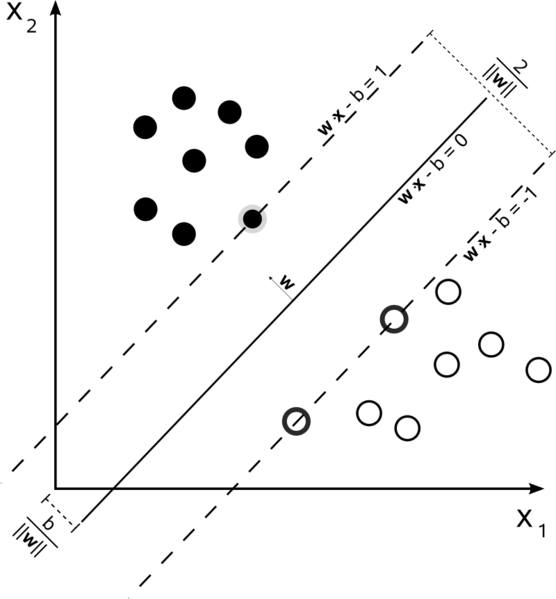
\includegraphics[width=0.8\linewidth]{figs/svm_margin.png}
\caption{Maximum-margin hyperplane and margins for an SVM trained with samples from two classes. Samples on the margin are called the support vectors. \textbf{b} stands for margin.}
\end{figure}
\paragraph{The Hyperplane}
The perpendicular distance of a point x from a hyperplane defined by $f(x)=0$ where $f(x)=w^T \phi(x) + w_0$ is given by $\frac{|f(x)|}{\parallel w \parallel}$. Furthermore we're only interested in a solution where all points are correctly classified. Thus the distance of a point $x_i$ to the decision surface becomes
\begin{align}
\frac{y_i f(x_i)}{\parallel w \parallel}=\frac{y_i(w^T \psi(x_i) + w_0)}{\parallel w \parallel}
\end{align}
The maximum margin solution is given by
\begin{align}
\argmax_{w, w_0} \{\frac{1}{\parallel w \parallel} \min_i[y_i (w^T\psi(x_i) + w_0)]\}
\end{align}
where we have taken factor $\frac{1}{\parallel w \parallel}$ outside of the optimization because $w$ doesn't depend on $i$. Direct solution of this problem would be very complex, therefore we simplify it. We notice that if we rescale $w \rightarrow \gamma w$ and $w_0 \rightarrow \gamma w_0$ then the distance from any $x_i$ to decision surface given by $frac{y_i f(x_i)}{\parallel w \parallel}$ doesn't change. Therefore
\begin{align}
y_i (w^T\psi(x_i) + w_0) = 1
\end{align}
for the point that is closest to the surface. In this case all datapoints will satisfy
\begin{align}
y_i (w^T\psi(x_i) + w_0) \geq 1
\end{align}
This is called the \textbf{canonical representation} of the decision hyperplane. In case of points for which the constraints holds, the constraints are called active. Otherwise they're inactive. The optimization problem therefore requires to maximize $\parallel w \parallel^-1$ which is equivalent to minimizing $\parallel w \parallel^2$. The optimization problem becomes:
\begin{align}
\argmin_{w,w_0} \frac{1}{2} \parallel w \parallel^2 \\
subject \ to \ y_i (w^T\psi(x_i) + w_0) \geq 1 \ \forall_i
\end{align}
\paragraph{Lagrangian}
Now we reformulate this problems as a lagrange problem. The condition needs to be turned into the form $g(w) \geq 0$ and we add multipliers:
\begin{align}
L(w,w_0,\alpha)=\frac{1}{2}\parallel w \parallel^2 - \sum_i^N \alpha_i \{y_i (w^T\psi(x_i) + w_0) - 1\}
\end{align}
where $\alpha$ is a vector containing the lagrange multipliers for each training sample $i \in \{1, ... ,N\}$. The sign in front of the sum means that we're minimizing with respect to $w$ and $w_0$ and maximizing with respect to $\alpha$. Setting the derivatives of $L(w,w_0,\alpha)$ with respect to $w$ and $w_0$ equal to zero, we obtain the following two conditions:
\begin{align}
w = \sum_i \alpha_i y_i \psi(x_i) \\
0 = \sum_i \alpha_i y_i
\end{align}
\paragraph{Dual Problem}
We can now eliminate $w$ and $w_0$ from $L(w,w_0,\alpha)$ which gives us the dual representation of the maximum margin problem in which we maximize
\begin{align}
L(w,w_0,\alpha)=\frac{1}{2}\parallel w \parallel^2 - \sum_i^N \alpha_i \{y_i (w^T\psi(x_i) + w_0) - 1\} \\
\tilde{L}(\alpha)=\frac{1}{2} \sum_i^N \sum_j^N \alpha_i \alpha_j y_i y_j k(x_i, x_j) - \sum_i^N \sum_j^N \alpha_i \alpha_j y_i y_j k(x_i, x_j) + \sum_i^N \alpha_i \\
\tilde{L}(\alpha)=\sum_i^N \alpha_i - \frac{1}{2} \sum_i^N \sum_j^N \alpha_i \alpha_j y_i y_j k(x_i, x_j) \\
subject \ to \ constraints \ \alpha  \geq 0 \ \forall_i \\
\sum_i^N \alpha_i y_i = 0
\end{align}
Here the kernel function is defined by $k(x, x')=\psi(x)^T \psi(x')$.
To evaluate new data points we use
\begin{align}
f(x)=\sum_i^N \alpha_i y_i k(x, x_i) + w_0
\end{align}
Since usually only a small minority of data points are support vectors, most $\alpha_i=0$. For the support vectors holds $y_if(x_i) = 1$. Therefore the evaluation is computationally simple, because the non-support vectors can be discarded after training. \newline
\paragraph{Evaluating Data Points}
To calculate $w_0$ we use the fact that for any support vector $y_if(x_i) = 1$. Using $f(x)=\sum_i^N \alpha_i y_i k(x, x_i) + w_0$ we obtain:
\begin{align}
y_i(\sum_{j \in \mathcal{S}} \alpha_j y_j k(x_i, x_j) + w_0) = 1
\end{align}
where $\mathcal{S}$ is the set of support vectors. Using $y_i^2=1$ we get
\begin{align}
w_0=\frac{1}{N_{\mathcal{S}}} \sum_{i \in \mathcal{S}} (y_i - \sum_{j \in \mathcal{S}} \alpha_j y_j k(x_i, x_j))
\end{align}
which is numerically more stable and where $N_{\mathcal{S}}$ is the total number of support vectors.
\subsection{Soft margin SVMs}
So far we assumed that the data points are linearly separable. Now we consider the case where the classes overlap, which is usually the case in practice. Therefore we introduce a method to allow some data points to be inside the margin or even on the wrong side of the separating hyperplane. To do this we use slack variables $\xi_i \geq 0$ for each data point which gives a measure of the misclassification of data point $i$.these are defined by $\xi_i = 0$ for data points on or inside the correct margin boundary and $\xi_i=|y_i - f(x_i)|$ for other points. Thus points on the separating hyperplane will have $\xi_i=1$ and misclassified datapoints will have $\xi_i > 1$. The exact misclassification constraints are then replaced with 
\begin{align}
y_i f(x_i) \geq 1 - \xi_i \ \forall_i
\end{align}
These are called sometimes relaxation constraints and an SVM using these is known as a \textbf{Soft margin SVM}. Our goal is now tho maximize the margin while softly penalizing points lying on the wrong side of the margin boundary. We therefore optimize
\begin{align}
C \sum_i^N \xi_i + \frac{1}{2} \parallel w \parallel^2
\end{align}
where $C>0$ weights the impact of the slack penalties on the final result.
We turn this into a Lagrangian:
\begin{align}
L(w,w_0,\xi,\alpha,\beta)=\frac{1}{2}\parallel w \parallel^2+C \sum_i^N \xi_i-\sum_i^N \xi_i \{y_i f(x_i)-1 + \xi_i\}-\sum_i^N \beta_i \xi_i
\end{align}
where $\alpha_i \geq 0$ and $\beta_i \geq 0$ are Lagrange multipliers. The corresponding KKT conditions are given by
\begin{align}
\alpha_i \geq 0 \\
y_i f(x_i)-1+\xi_i \geq 0 \\
\alpha_i(y_i f(x_i)-1+\xi_i) = 0 \\
\beta_i \geq 0 \\
\xi_i \geq 0 \\
\beta_i \xi_i = 0
\end{align}
We now optimize out $w$, $w_0$ and $\xi$ using $f(x)=w^T\psi(x)+w_0$
\begin{align}
\frac{\partial L}{\partial w}=0 \Rightarrow w=\sum_i^N\alpha_i y_i\psi(x_i) \\
\frac{\partial L}{\partial b}=0 \Rightarrow \sum_i^N\alpha_i y_i = 0 \\
\frac{\partial L}{\partial \xi_i}=0 \Rightarrow \alpha_i=C-\beta_i
\end{align}
using these to eliminate $w$, $w_0$ and $\xi$ we obtain the dual Lagrangian in the form
\begin{align}
L(w,w_0,\xi,\alpha,\beta)=\frac{1}{2}\parallel w \parallel^2 + C \sum_i^N \xi_i - \sum_i^N \alpha_i \{y_i (w^T\psi(x_i) + w_0) - 1 + \xi_i\} - \sum_i^N \beta_i \xi_i \\
L(w,w_0,\xi,\alpha,\beta)=\frac{1}{2} \sum_i^N \sum_j^N \alpha_i \alpha_j y_i y_j k(x_i, x_j) + C \sum_i^N \xi_i - \sum_i^N \sum_j^N \alpha_i \alpha_j y_i y_j k(x_i, x_j) + \sum_i^N \alpha_i(1-\xi_i) - \sum_i^N \beta_i \xi_i \\
L(w,w_0,\xi,\alpha,\beta)= \sum_i^N \alpha_i - \frac{1}{2} \sum_i^N \sum_j^N \alpha_i \alpha_j y_i y_j k(x_i, x_j) + \sum_i^N (C - \alpha_i - \beta_i) \xi_i \\
ignoring: \ C - \alpha_i - \beta_i = \frac{\partial L}{\partial \xi_i} = 0 \\
\tilde{L}(\alpha)=\sum_i^N \alpha_i - \frac{1}{2} \sum_i^N \sum_j^N \alpha_i \alpha_j y_i y_j k(x_i, x_j)
\end{align}
We notice that the Lagrangian looks the same as for the Hard Margin case. The difference lies in the constraints that are somewhat different. We note that $\alpha_i \geq 0$ is required because they're Lagrange multipliers. Furthermore $\alpha_i=C-\beta_i$ together with $\beta_i \geq 0$ implies that $\alpha \leq C$. We therefore maximize with respect to $\alpha$ subject to
\begin{align}
0 \leq \alpha_i \leq C \\
\sum_i^N \alpha_i y_i = 0
\end{align}
where the first kind of constraints are known as the box constraints. Prediction of new data points are made like in the Hard Margin SVM. As before a subset of the data points may have $\alpha_i=0$ in which case they don't contribute to the predictions. The remaining data points constitute the support vectors. These have $\alpha_i>0$ and from $\alpha_i(y_i f(x_i)-1+\xi_i) = 0$ must satisfy
\begin{align}
y_i f(x_i)=1-\xi_i
\end{align}
If $\alpha_i<C$ then $\alpha_i=C-\beta_i$ implies that $\beta_i>0$, which according to $\beta_i \xi_i = 0$ requires $\xi_i=0$ and hence such points lie on the margin. Points with $\alpha = C$ can lie inside the margin and can be either correctly classified if $\xi_i \leq 1$ or misclassified if $\xi_i > 1$. To determine $w_0$ we note that support vectors for which $0<\alpha_i<C$ have $\xi_i=0$ so that $y_i f(x_i)=1$ and hence will satisfy
\begin{align}
y_i(\sum_{j \in \mathcal{S}} \alpha_j y_j k(x_i, x_j) + w_0) = 1
\end{align}
like in the Hard Margin SVM case. Again, a numerically more stable solution is given by
\begin{align}
w_0=\frac{1}{N_{\mathcal{M}}} \sum_{i \in \mathcal{M}} (y_i - \sum_{j \in \mathcal{M}} \alpha_j y_j k(x_i, x_j))
\end{align}
where $\mathcal{M}$ is the set of indices of data points satisfying $0<\alpha_i<C$.
\subsection{Readings}
\begin{enumerate}
\item SVM: Bishop, Chapter 7.1
\item Lagrange multipliers: Bishop, Appendix E
\item Slides from Lecture 8
\end{enumerate}
\end{document}